\section{Evaluating the Harness}
\label{sec:evaluation}

\subsection{Scale and storage}

Table~\ref{tab:models_calls} reports the delivered call budget per model. The total is 275,218 calls, written to 39 prediction files totaling 0.489\,GiB. The matrix has zero error rows: every row is either a parsed reply or a captured parse failure, not a lost call. The largest single file is 66.7\,MB (MedGemma-1.5 shift), which is small enough that all audits can stream it on a laptop. The companion measurement paper additionally reports a 400-study LLaVA-Med NIH subset outside this 39-file harness matrix; the all-inclusive count including that subset is 275,618 calls (270,324 six-model matrix plus 5,294 LLaVA-Med).

\begin{table}[t]
\centering
\small
\caption{Delivered calls and prediction footprint per model. Call counts are exact JSONL row counts; storage is the sum of the frozen prediction files.}
\label{tab:models_calls}
\begin{tabular}{lrr}
\toprule
Model & Calls & Prediction size (MiB) \\
\midrule
MedGemma-4B & 60,616 & 104.1 \\
MedGemma-1.5 & 45,556 & 114.3 \\
Qwen2.5-VL & 45,556 & 81.9 \\
Qwen3-VL & 39,532 & 71.9 \\
InternVL3.5 & 39,532 & 69.1 \\
CheXagent & 39,532 & 56.9 \\
LLaVA-Med & 4,894 & 2.8 \\
\midrule
Total & \textbf{275,218} & \textbf{501.0} \\
\bottomrule
\end{tabular}
\end{table}

\subsection{Durability has a measured price}

Table~\ref{tab:cost} runs five writers over the same 2,000-cell workload: the same
keys, the same 1.52\,kB payload, the same machine, no GPU. The shipped writer is
the slowest of the four durable options and the only one that is slower than a
per-row fsync, because it fsyncs both the prediction file and its sidecar. That
cost is real: 1.95\,ms per cell against 0.003\,ms for a naive append.

It is also small where it matters. The delivered matrix took about 231 GPU-hours,
roughly ten days; at 275,218 calls the durability guarantee adds about nine
minutes. A study that cannot afford nine minutes of fsync cannot afford the GPU
stage it is protecting. The honest reading is therefore not ``durability is free''
but ``durability is cheap relative to the thing it makes repeatable''.

One baseline needs an explicit caveat. B2 buffers 100 cells and rewrites the whole
file atomically, so its 0.000\,ms p50 measures only the in-memory insert; the
rewrite cost sits in the p99 (0.032\,ms) and is invisible at 2{,}000 cells. At the
scale of this study it is not viable: 275,218 cells would trigger about 2{,}750
rewrites averaging 137{,}600 rows, roughly 209\,MB each and some 576\,GB written in
total. B2 is therefore a micro-batch baseline, included because it is the design
that multimodal evaluation kits effectively use at file granularity, not a
candidate for a 275k-call job.

\begin{table}[t]
\centering
\small
\caption{The price of durability, 2{,}000 cells, 1.52\,kB per row, CPU only, no
faults. Append latency is per cell; recovery is the time to rebuild the completed-key
set from the artefact. SQLite is the only baseline whose per-row storage differs,
because it stores typed pages rather than text. B2's p50 is an in-memory insert;
its flush cost appears in the p99. B2 is a micro-batch baseline and is not viable
at 275k cells (Section~\ref{sec:evaluation}, limitations).}
\label{tab:cost}
\begin{tabular}{llrrrrr}
\toprule
Writer & Mechanism & Cells/s & p50 (ms) & p99 (ms) & B/row & Recover (s) \\
\midrule
B0 & append, no fsync & 200{,}184 & 0.003 & 0.019 & 1{,}522 & 0.013 \\
B1 & append + fsync per row & 2{,}218 & 0.429 & 0.759 & 1{,}522 & 0.014 \\
B2 & rewrite whole file, atomic & 15{,}393 & 0.000 & 0.032 & 1{,}522 & 0.013 \\
B3 & SQLite, WAL, commit per batch & 54{,}797 & 0.004 & 0.052 & 2{,}091 & 0.002 \\
\textbf{B4} & \textbf{shipped: append + fsync + sidecar} & \textbf{501} & \textbf{1.954} & \textbf{2.726} & \textbf{1{,}521} & \textbf{0.010} \\
\bottomrule
\end{tabular}
\end{table}

\subsection{Durability has a measured payoff}

Table~\ref{tab:faults} injects ten faults at the operating-system boundary ---
the syscall the guarantee actually rests on --- rather than describing what the
code is supposed to do. Every fault is attempted against every writer that has a
mechanism for it; a cell marked n/a means the baseline has no such mechanism, not
that it passed.

Four results matter. (i) A crash loses 10 of 700 cells under naive append (1.4\%)
and none under any durable writer. (ii) Concurrency separates the field into
three behaviours: append and append\,+\,fsync silently duplicate keys (505 and
700); the atomic-rewrite and sidecar writers refuse loudly; SQLite, which has
real locking, handles both writers cleanly and ends with zero duplicates. We
report this as a genuine advantage of B3 over B4, not as a mechanism it lacks.
(iii) No writer silently reports success when write, fsync or rename fails; every
applicable cell raises. (iv) A corrupted sidecar, or a sidecar whose offset is
ahead of the file, costs the shipped writer zero rows --- recovery re-reads the
JSONL rather than trusting the sidecar.

\begin{table}[t]
\centering
\footnotesize
\setlength{\tabcolsep}{4pt}
\caption{Fault injection, 700 cells attempted against a 2{,}000-cell target.
``lost'' is cells reported written but not recoverable; ``dup'' is duplicate keys
after recovery; ``raised'' means the writer surfaced the failure instead of
claiming success. n/a: the mechanism does not exist in that writer. $\dagger$:
byte-level fault injection cannot reach SQLite's C file layer, so B3's I/O cells
are untested rather than passed; B3 is tested on crash, torn tail, concurrency and
read-only.}
\label{tab:faults}
\begin{tabular}{lccccc}
\toprule
Fault injected & B0 & B1 & B2 & B3 & \textbf{B4} \\
\midrule
process crash (700 cells) & 10 lost & 0 & 0 & 0 & \textbf{0} \\
truncated tail & 1 lost & 1 lost & 1 lost & n/a & \textbf{1 lost} \\
two concurrent writers & 505 dup & 700 dup & refused & \textbf{clean} & refused \\
write failure (ENOSPC) & raised & raised & raised & n/a$\dagger$ & \textbf{raised} \\
fsync failure & n/a & raised & raised & n/a$\dagger$ & \textbf{raised} \\
rename failure & n/a & n/a & raised & n/a$\dagger$ & \textbf{raised} \\
sidecar corrupted & n/a & n/a & n/a & n/a & \textbf{0 lost} \\
sidecar offset ahead & n/a & n/a & n/a & n/a & \textbf{0 lost} \\
file made read-only & refused & refused & refused & refused & \textbf{refused} \\
configuration changed & n/a & n/a & n/a & n/a & \textbf{refused} \\
\bottomrule
\end{tabular}
\end{table}

\subsection{Five invariants replace ``zero error rows''}

A benchmark-engineering paper typically claims zero error rows. That claim is not
falsifiable: if every failure is written as a row, the count is zero by
construction. The measured matrix supports five statements that can fail:
\begin{enumerate}[leftmargin=1.4em,itemsep=1pt,topsep=2pt]
\item \textbf{Unique keys.} A single writer never emits the same
(image, condition, severity) twice. All five satisfy this; two concurrent writers
break it for B0 and B1 and are refused by B2 and B4.
\item \textbf{No acknowledged-row loss.} A cell that the process counted as done
survives a crash. B0 fails (10/700); B1--B4 pass.
\item \textbf{No silent I/O success.} Injected write, fsync and rename failures
surface as exceptions. All five pass.
\item \textbf{No torn tail accepted as complete.} After truncation every file
exposes the regression as 699 of 700. What this does and does not show matters:
the writers do not self-detect the tear --- none of them carries an expected
count --- so the invariant is about the artefact being auditable, not about the
writer being self-checking. The audit knows the denominator; the writer does not.
\item \textbf{No silent configuration mixture.} A resumed stage whose prompt,
label set, manifest or runner hash changed is refused. Only B4 implements this.
\end{enumerate}

\subsection{A denominator census that can fail}

The census recomputes each file's denominator from the file. For every prediction
file it reports rows, unique keys, duplicates, distinct images, the minimum and
maximum number of cells per image, parse failures and a content hash. A file whose
cells-per-image varies is not necessarily wrong, but the variation must be
declared: undeclared raggedness is what makes a published denominator
unreconstructible.

Applied to the full artefact tree --- 259 prediction files, 456,790 rows,
0.87\,GiB --- the census finds 255 files with a uniform denominator, four
non-uniform, and one with duplicate keys. Because an undeclared anomaly reads as
an accusation, every flag is declared here.

The duplicate file is \texttt{analysis\_round2/thinking\_invalid\_archive.jsonl}
(4{,}283 rows, 1{,}522 duplicate keys, parse rate 0.000). It is an archive of
non-terminating replies: the same cell can be retried and archived several times,
so duplicates are the intended structure, not corruption. It is outside the
39-file harness matrix.

{\sloppy
The four non-uniform files are also declared. The archive above is one. The second,
\texttt{bs\_sweep/bs4567}, is empty (0 rows) and is a truncated sweep artefact that
should be removed rather than analysed. The third,
\texttt{matrix/nih\_eval/qwen3\_vl\_8b\_thinking/shift}, holds 9{,}401 rows over
1{,}506 studies with 2--7 cells per study: a thinking checkpoint that never
terminates removes cells, and the paper reports the resulting 89.2\% usable
coverage explicitly. The fourth, \texttt{rrg/medgemma/rrg\_predictions.jsonl},
holds 314 rows over 264 studies with 1--2 cells, because the report-generation
layer carries one or two reference reports per study.\par}

None of the four is inside the 39-file matrix, so no denominator in the companion
paper is affected. This is the point of the census: the audit reports what it
finds, and the authors owe a declaration for each finding. The same procedure is
defined for any JSONL prediction file and does not depend on this harness having
produced it.

\subsection{Reliability}

The crash/resume suite passes 40/40 checks (Table~\ref{tab:resume}). The authoritative package also has unit tests for the parser, metrics, and durable writer: valid JSON, markdown fences, missing findings, invalid probabilities, label completeness, perfect/chance AUROC, ECE, append/resume, in-place replacement, and torn-tail truncation. These tests run in about one second on CPU.

The delivered matrix itself has no inference failures, but it does contain parse failures: CheXagent's NIH shift parse rate is 98.5\%, and MedGemma-1.5's is 99.8\%. Those are not hidden as ``missing''; they are rows with \texttt{parse\_success=false} and a \texttt{parse\_error}, counted in the census (Table~\ref{tab:coverage}). The distinction matters: a parse failure is evidence about the model's contract behavior, while a lost call is evidence about the harness.

\subsection{Batch size is a measurement parameter}

Throughput is not monotone in batch size, and the collapse is silent: no out-of-memory error, just a 2--16$\times$ slowdown as the driver pages memory over PCIe. Figure~\ref{fig:batch} and Table~\ref{tab:batch} show the measured curves. The harness chooses the smallest batch within 5\% of the best measured throughput, not the largest batch that fails to raise an error.

\begin{figure}[t]
\centering
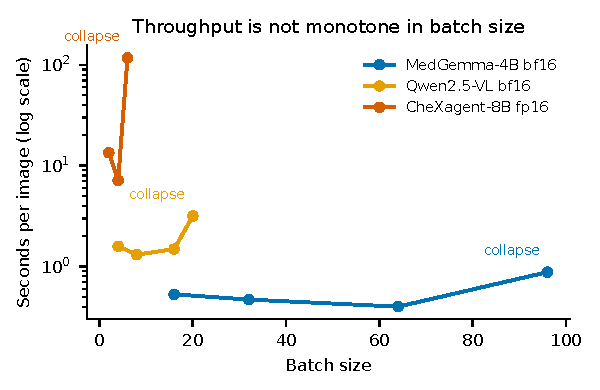
\includegraphics[width=0.82\textwidth]{figures/fig3_batch.pdf}
\caption{Measured throughput vs.\ batch size on an RTX 4080 SUPER 32\,GB under Windows WDDM. Each series ends at a silent collapse: GPU utilisation is high, power draw is far below the board limit, and per-image time rises sharply without an exception.}
\label{fig:batch}
\end{figure}

\begin{table}[t]
\centering
\small
\caption{Measured batch operating points (selected rows from the sweep). The last row of each block is the collapse point.}
\label{tab:batch}
\begin{tabular}{llrrr}
\toprule
Model & Precision & Batch & s/img & VRAM peak \\
\midrule
MedGemma-4B & bf16 & 16 & 0.53 & 12.6 \\
MedGemma-4B & bf16 & 64 & \textbf{0.40} & 21.0 \\
MedGemma-4B & bf16 & 96 & 0.88 & 26.6 \\
Qwen2.5-VL & bf16 & 4 & 1.59 & 16.7 \\
Qwen2.5-VL & bf16 & 8 & \textbf{1.31} & 18.1 \\
Qwen2.5-VL & bf16 & 20 & 3.17 & 29.7 \\
CheXagent & fp16 & 2 & 13.43 & 28.9 \\
CheXagent & fp16 & 4 & \textbf{7.14} & 29.7 \\
CheXagent & fp16 & 6 & 117.11 & 30.9 \\
\bottomrule
\end{tabular}
\end{table}

At equal batch size, 4-bit is within 2.5\% of bf16 throughput for MedGemma while using 6.8\,GB less VRAM (0.41 vs.\ 0.40\,s/img at batch 64; 14.2 vs.\ 21.0\,GB). Quantization is therefore not an accuracy-versus-speed trade-off on this hardware; it is a memory trade-off, and its effect on the \emph{findings} must be tested separately (the harness does so with a bf16 control).
